\documentclass{article}
\usepackage[utf8]{inputenc}
\usepackage[english]{babel}
\usepackage{amsmath}
\usepackage{natbib}
\usepackage{graphicx}
\usepackage{hyperref}

\begin{document}

{\centering

\rule{\textwidth}{1.6pt}\vspace*{-\baselineskip}\vspace*{2pt} 
\rule{\textwidth}{0.4pt}\\[\baselineskip] 
{\LARGE Growing Degree Day}
\rule{\textwidth}{0.4pt}\vspace*{-\baselineskip}\vspace{3.2pt}
\rule{\textwidth}{1.6pt}\\[\baselineskip] 

\vspace{20mm} %5mm vertical space
\scshape % Small caps
CMSC 6950 - Computer Based Research Tools and Applications \\ [\baselineskip]
Extended Assignment \\[\baselineskip] 
13th June, 2016 \\[\baselineskip] 
\vspace{20mm} %5mm vertical space
Submitted by \\[\baselineskip]
{\Large Mohammad Hassan \\ Ernest Awoonor-Williams \\ Mehrzad \\ Yin Zhang \\ Rufai raji \\ Lutfor Rahman \\ Mohammad Sheykholeslam\par}
\vfill
{\itshape Memorial University of Newfoundland \\ St. John's, Canada.\par} 
}

\newpage

{\centering
  \section*{Abstract}
}

{\itshape In this report, we calculated the growing degree days (GDD) based on different Canadian city's weather history. Three major cities were considered, namely: St. John’s, Calgary, and Montreal. The data collected was for the year 2015. The calculated GDD varies among the three cities considered. The city of Montreal had the largest GDD of 1448 $^{\circ}$C among the cities compared for GDD values recorded in that year. St. John's recorded the lowest GDD value of 501 $^{\circ}$C while the city of Calgary recorded a moderate GDD value of 796 $^{\circ}$C.\\
}

%\newpage
%\tableofcontents
%\newpage

\section{ \bf Introduction}
Growing degree days (GDD) is simply a predictive tool used in horticulture for accessing crop maturity and development. This predictive tool is helpful in providing adequate knowledge for timing the important growth stages of plants, as well as in assessing the suitability of a region for growing specific crops of interest. As such, GDD units are a frequently used weather-based indicator for plant development assessment. The GDD calculation within a period of time is dependent on heat accumulation and is typically measured from the start of the growth cycle of a plant. It is usually defined relative to a base reference temperature which varies among crops based on their life cycles. The total GDD over a growing season is related to plant development. The development of plants depends on the accumulation of heat. Since cool season plants have a lower reference temperature, they accumulate GDDs faster than warm season plants. Unless plants are overly stressed by drought or pests, the total GDDs can be used to predict when a crop will reach maturity. Corn, for example, requires 1360 GDD units to mature. GDDs can be computed using climatic information for any location. That computation, along with data on soil, water, and minimum and maximum temperatures, helps suggest which crops will grow best in a given region.\\ [\baselineskip] GDD has units of temperature (i.e., $^{\circ}$C or $^{\circ}$F) and is calculated by subtracting the base temperature from the average of the daily temperatures (i.e. maximum and minimum temperatures). The equation for calculating the GDD, Eqn.(\ref{eqn:gdd}), is given as follows:

\begin{equation}
\textrm{GDD} = \left(\frac{T_{max} + T_{min}}{2}\right) - T_{base}
\label{eqn:gdd}
\end{equation}

\noindent where {$T_{max}$} is the daily maximum temperature and {$T_{min}$} is the daily minimum temperature. {$T_{base}$} is the base temperature, which is the minimum temperature required for the growth of a particular crop. For the GDD calculations reported in the study, {$T_{base}$} is considered to be 10 $^{\circ}$C.\\
In this report, we present a summary of the results obtained from calculating the annual GDD in 2015 for three cities in Canada; namely: St. John's, Montreal and Calgary. As expected, the calculated GDDs varies for the selected cities. 


\section{ \bf Methodology}
\subsection{Data Collection}
The data for the daily historical temperatures for the selected cities were downloaded from: http://climate.weather.gc.ca. From the collected data, the minimum and maximum daily temperature values all year round were extracted for the selected cities. Daily GDD values were then computed and the results were analyzed and plotted as graphs. A summary of the approach adopted in data collection and analysis is presented below:

\begin{itemize}
\item Download daily historical data for the three selected cities. 
\item Calculate Daily GDD for cities within the time range selected. 
\item Compute Cumulative GDD for the cities within the selected time range.
\item Create a plot showing variations in annual GDD cycle for the chosen cities within the selected time range. 
\item Create a plot demonstrating accumulated GDD vs time for the chosen cities within the time frame selected. 
\end{itemize}

\subsection{Growing Degree Day Calculation}
Growing Degree Day (GDD) are calculated by taking the difference between the average daily temperatures and a threshold base temperature, $T_{base}$, (usually 10$^{\circ}$C). The equation for GDD calculation is as follows: \vspace{5mm}

\begin{equation}
\textrm{GDD} = \left(\frac{T_{max} + T_{min}}{2}\right) - T_{base}
\end{equation}

\noindent {$T_{max}$}, {$T_{min}$}, and {$T_{base}$} are the daily maximum, daily minimum and base temperatures, respectively. If the daily mean temperature is lower than the base temperature then $\textrm{GDD} = 0$.In other words, any temperature below $T_{base}$ is set to $T_{base}$ before calculating the average. GDDs are typically measured from the start of spring. A sample GDD calculation for a day in spring with a high of 20$^{\circ}$C and a low of 10$^{\circ}$C is evaluated as follows:\vspace{5mm}

\[ \left(\frac {20+10}{2}\right)-10=5 \] \par


\subsection{ \bf Core Project Tasks Completed}

\begin{enumerate}
\item  Automated download of daily historical temperature data for the selected cities based on station ID number
\item  Plots showing annual cycle of min/max daily temperatures for selected Canadian cities (Fig. \ref{gdd_min-max})

\begin{center}
\begin{figure}[!htb]
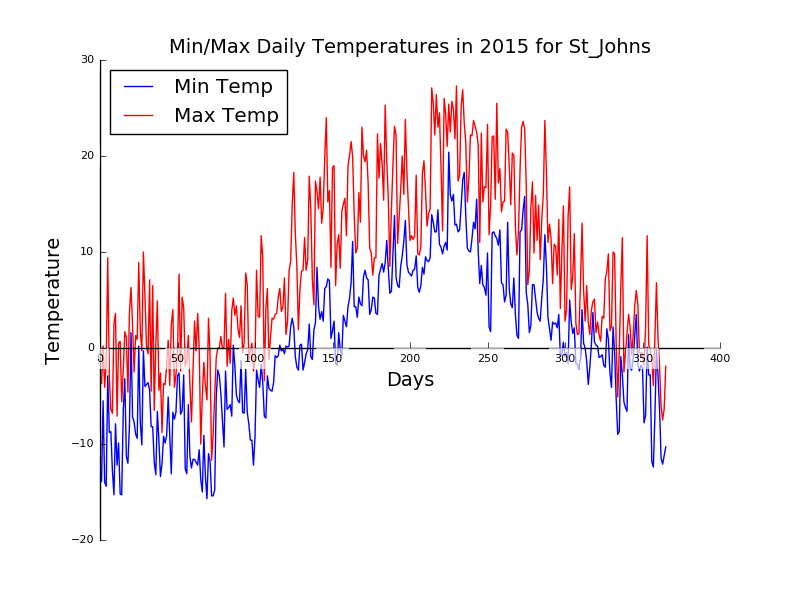
\includegraphics[width=3.25in]{./Plots/min_max_plot_St_Johns.png}

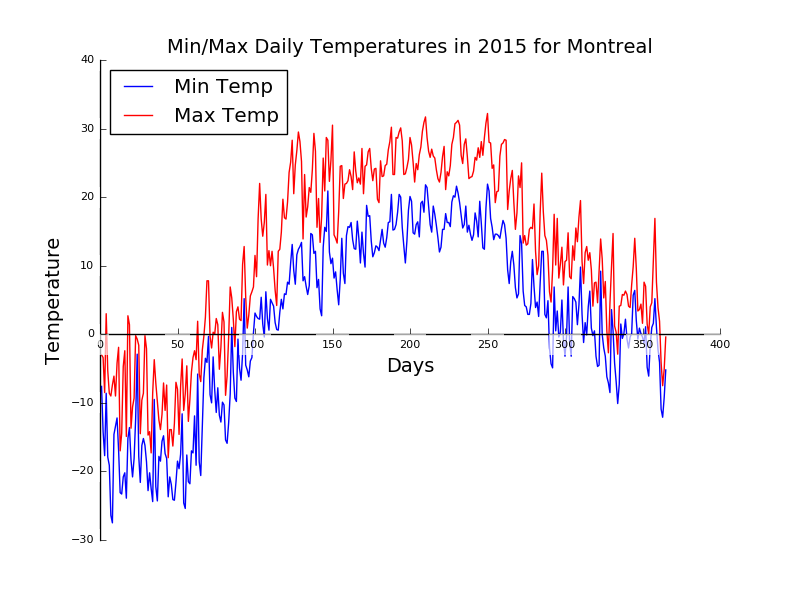
\includegraphics[width=3.25in]{./Plots/min_max_plot_Montreal.png}

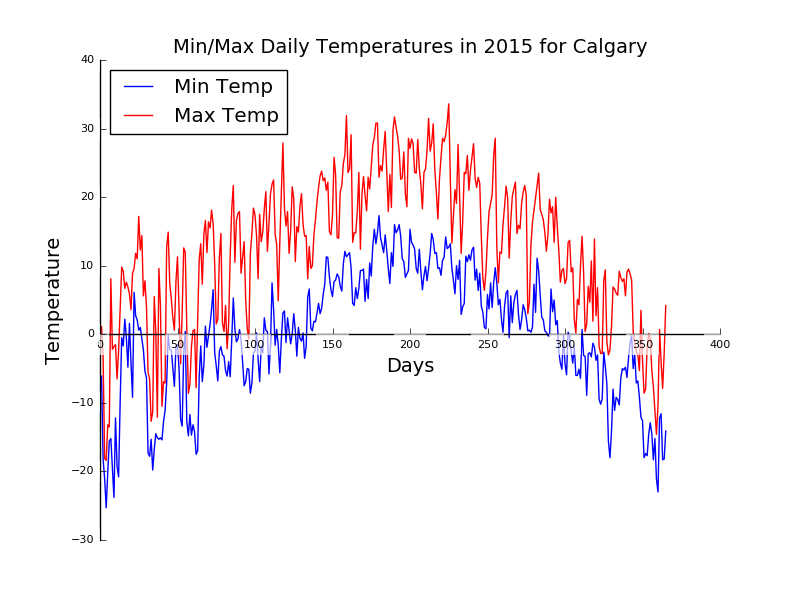
\includegraphics[width=3.25in]{./Plots/min_max_plot_Calgary.png}

\caption{Cycle of minimum and maximum daily temperatures in 2015 for selected cities.}
\label{gdd_min-max}
\end{figure}
\end{center}

\item  GDD calculation and storage for data analysis by a command line program
\item  Plots showing accumulated GDD versus time for selected cities (Fig. \ref{gdd_ann-cycle})

\begin{center}
\begin{figure}
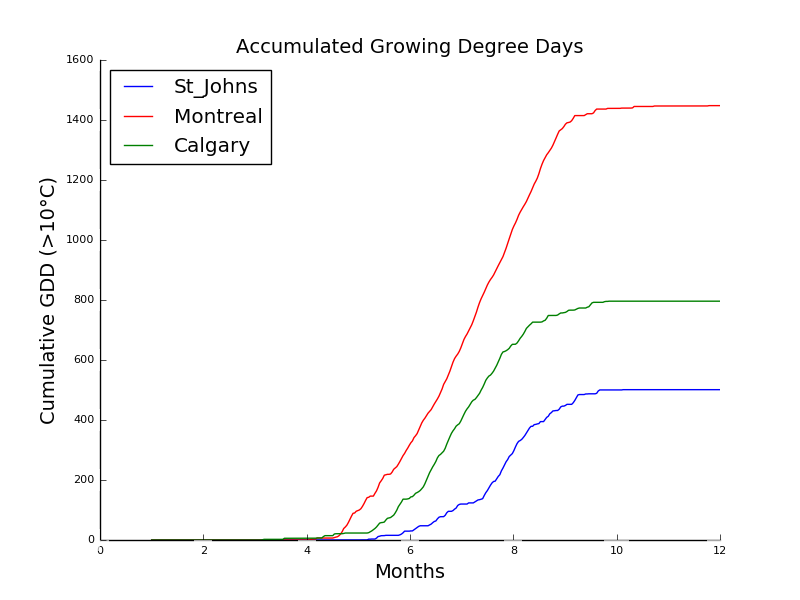
\includegraphics[width=3.25in]{./Plots/GDD_Plot.png}
\caption{2015 Annual cumulative GDD for selected cities.}
\label{gdd_ann-cycle}
\end{figure}
\end{center}

\end{enumerate}

%\subsection{Use version control (git) and collaboration tools (GitHub)}
%\subsection{Create a LaTeX report summarizing the results of your project}
%\subsection{Create a web based presentation for your results}
%\subsection{Implement your entire workflow as a Makefile. Ensure that your entire project is reproducible}
%\subsection{Create a test-suite (using the Python package nose) to demonstrate your GDD calculation works as intended}
%\subsection{Project should include adequate documentation both with your source code and Readme.md file}

\subsection{ \bf Optional Tasks Completed}
\begin{enumerate}
\item A bokeh plot showing GDD for selected Canadian cities considered (Fig. \ref{bokeh_min-max})
\begin{center}
\begin{figure}
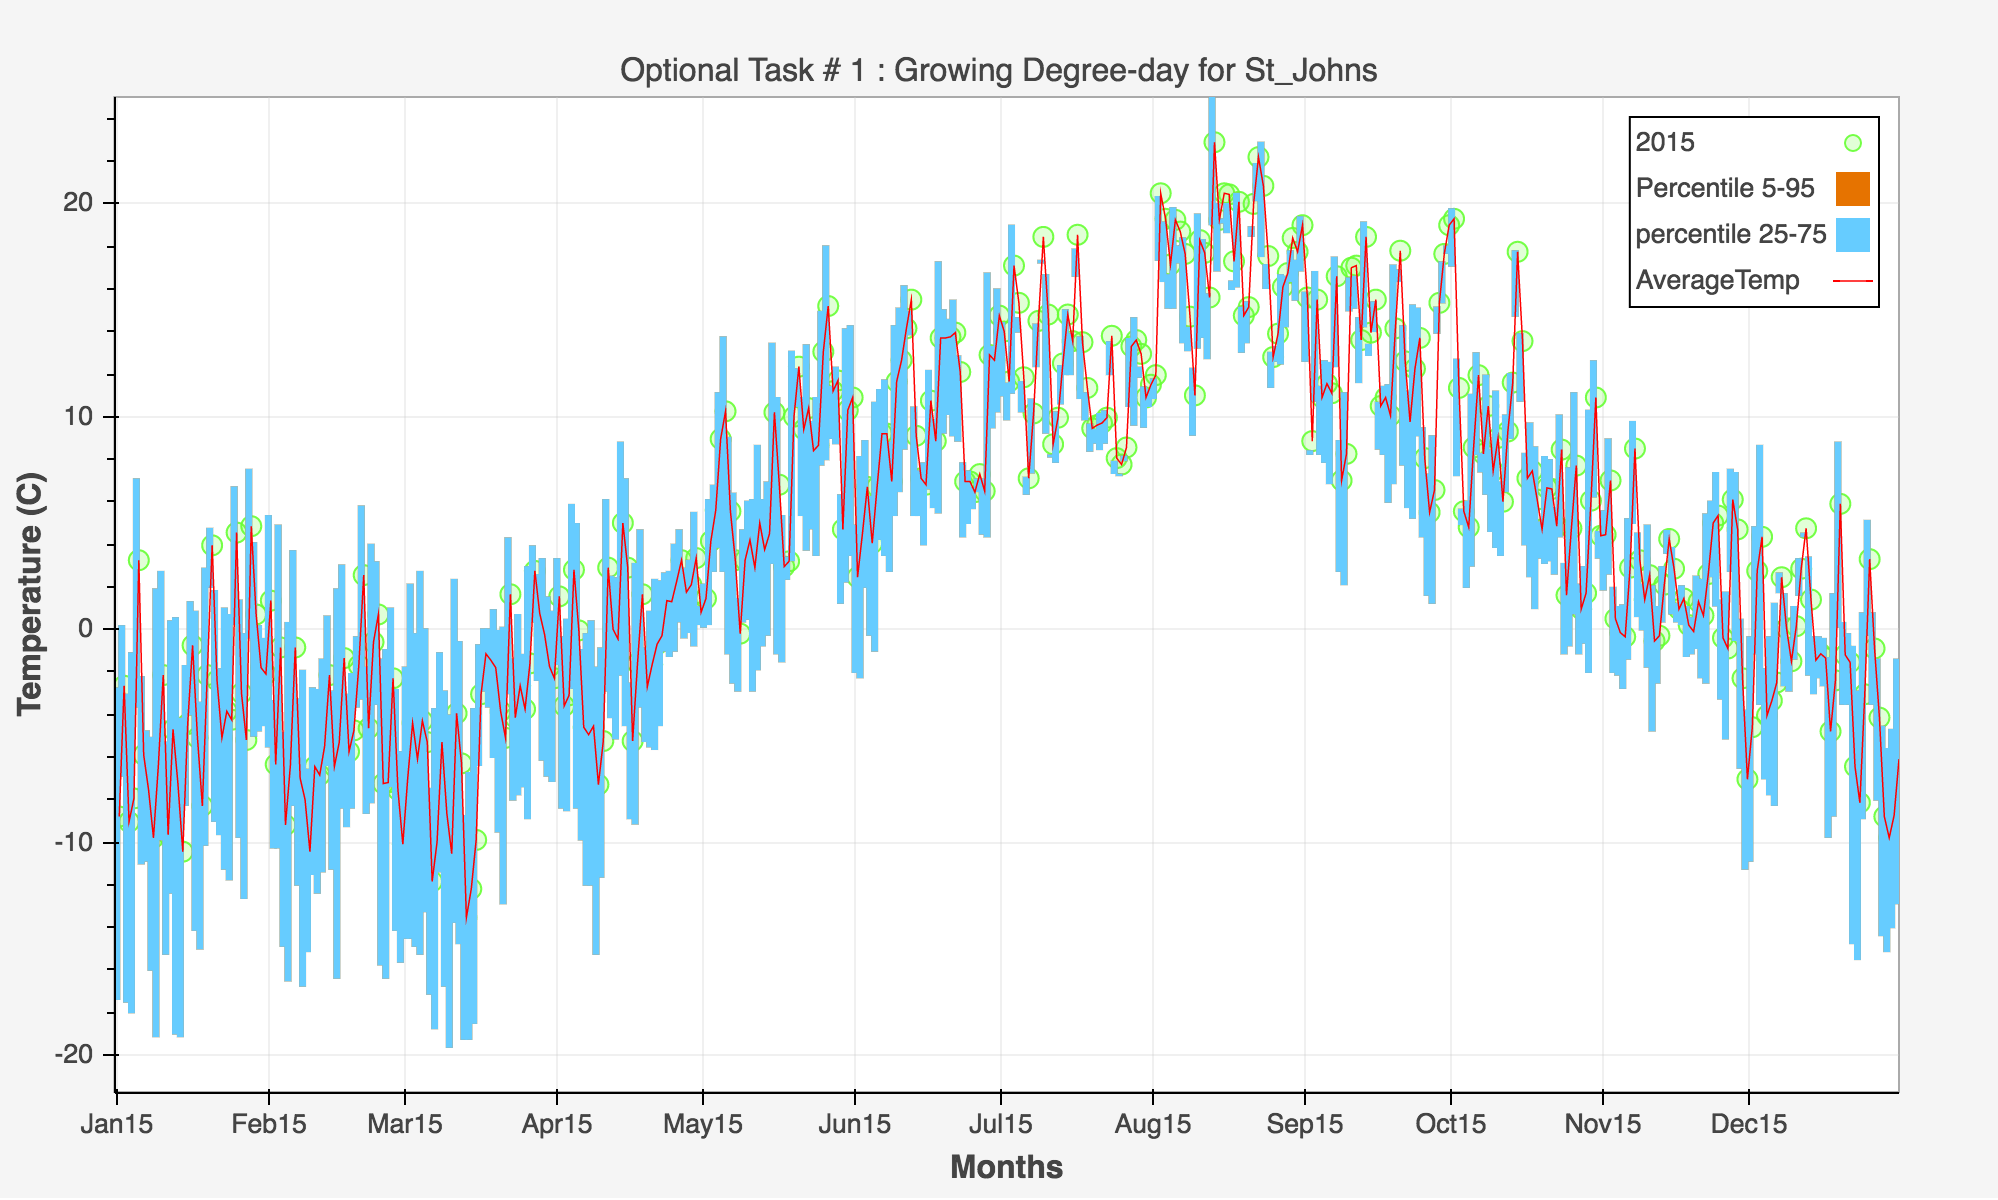
\includegraphics[width=3.25in]{./source/Report/op-task-1_st_johns.png}\\

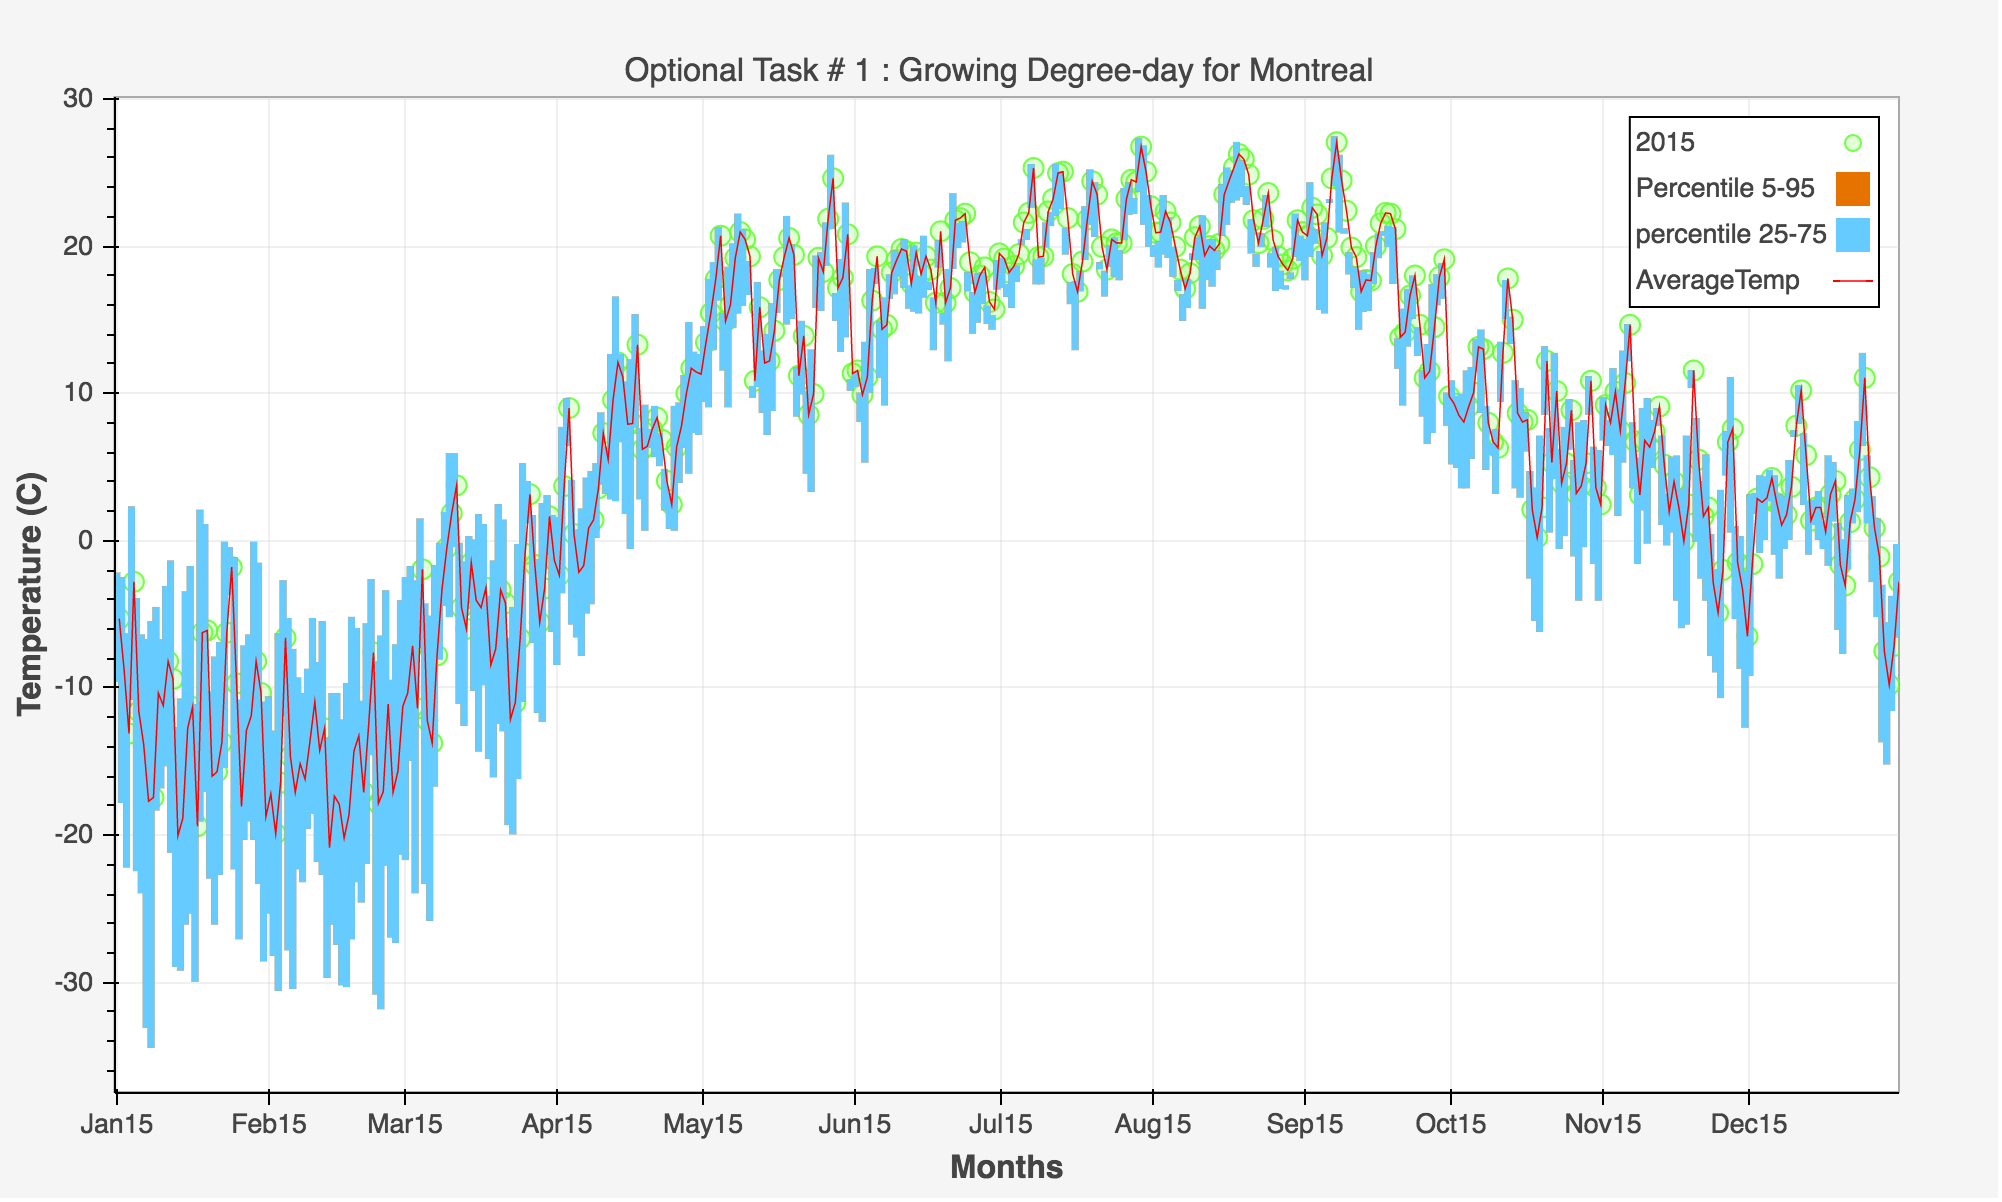
\includegraphics[width=3.25in]{./source/Report/op-task-1_montreal.png}\\

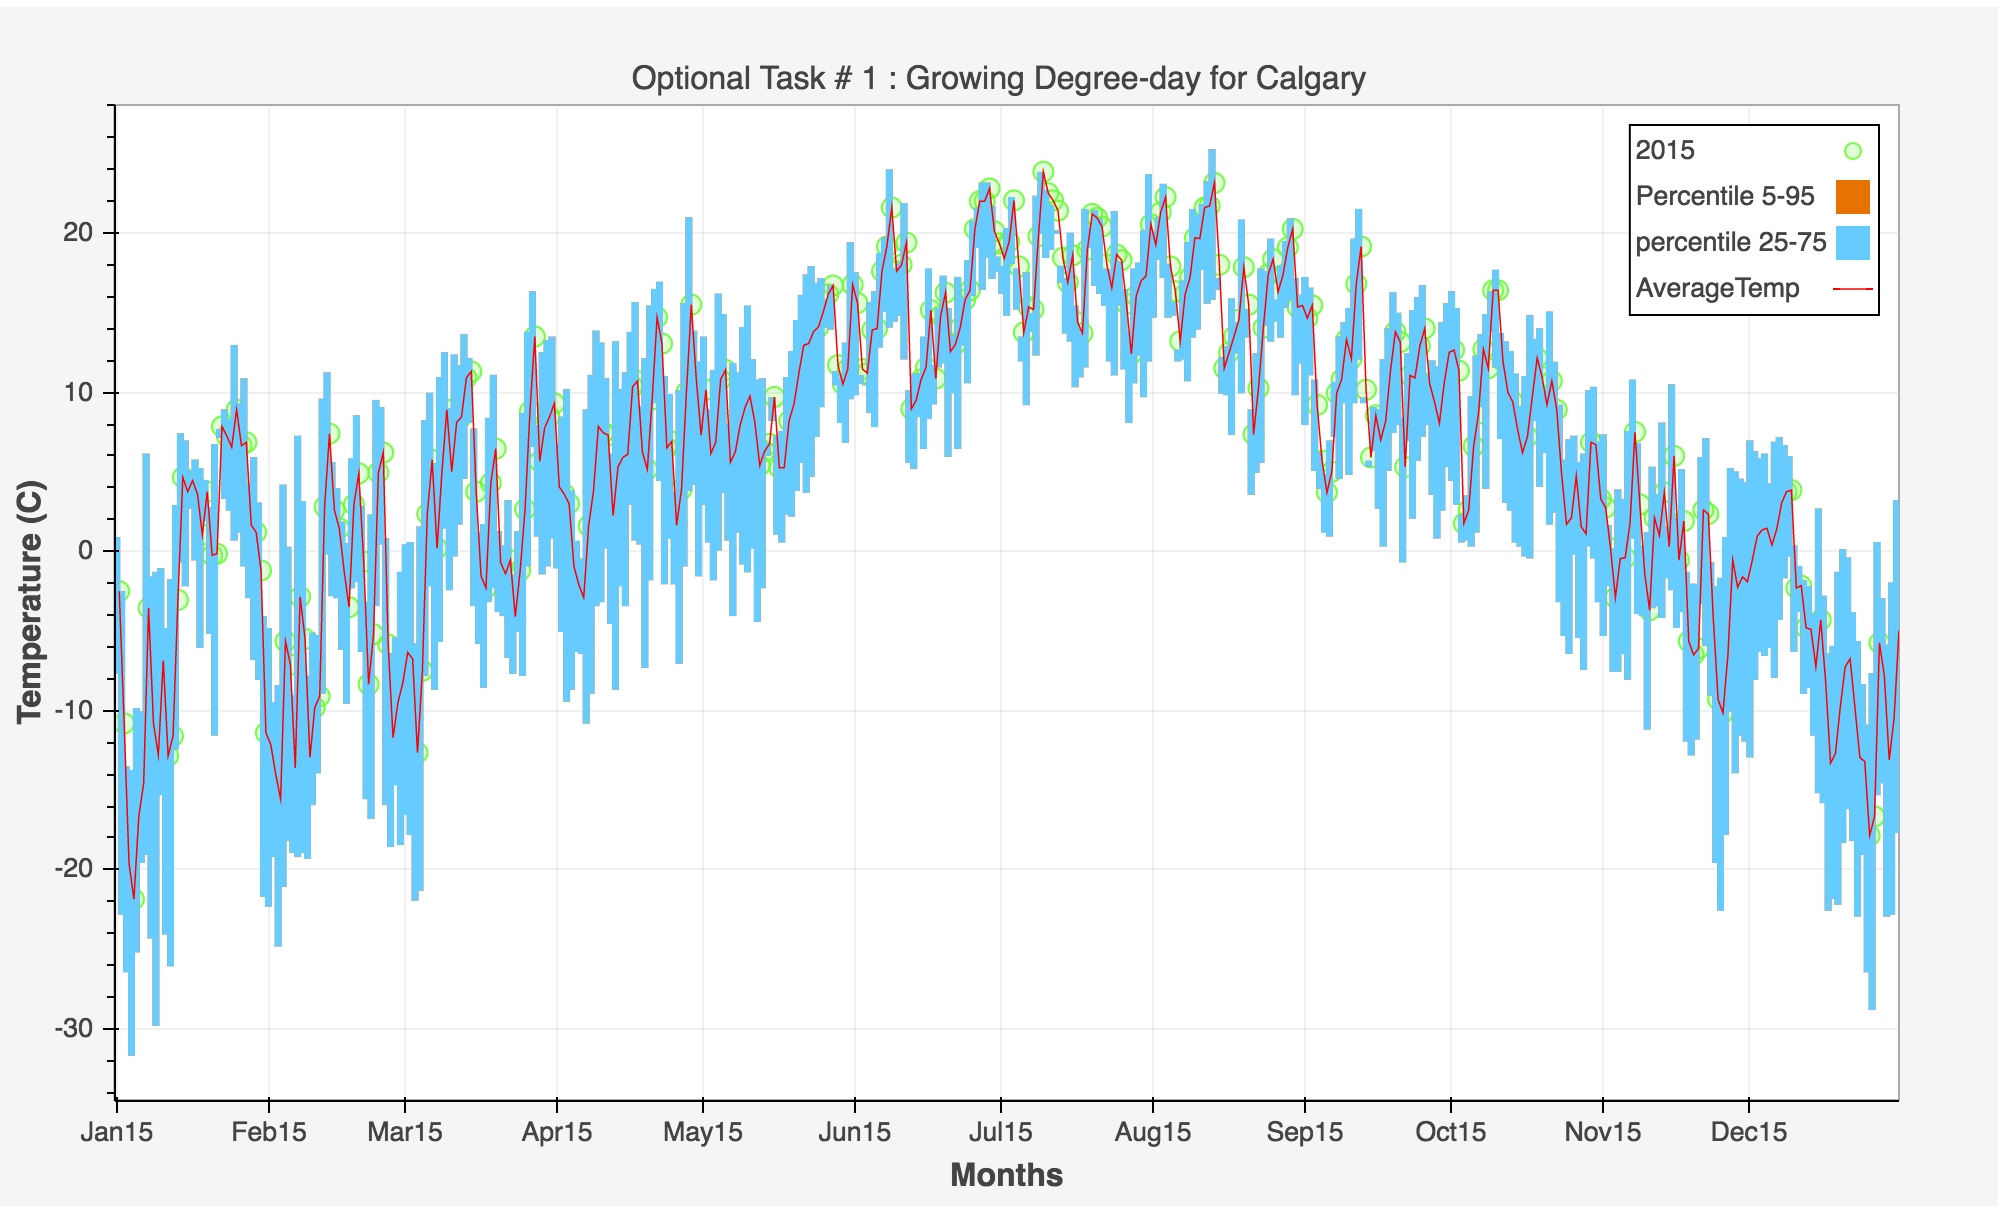
\includegraphics[width=3.25in]{./source/Report/op-task-1_calgary.png}\\

\caption{Bokeh plot displaying annual GDD min-max cycle for selected cities}
\label{bokeh_min-max}
\end{figure}
\end{center}
%\subsection{Create a map showing effective growing degrees over both all of Canada and only for the island of Newfoundland.}
\item Exploration of how GDD calculation depends on the choice of $T_{base}$ (Fig. \ref{gdd_diff-tbase})
\begin{center}
\begin{figure}
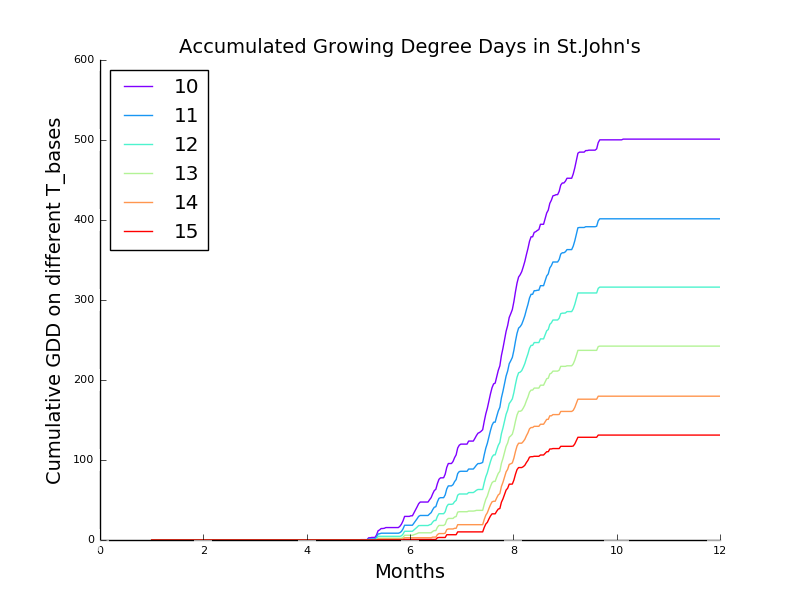
\includegraphics[width=3.25in]{./source/Report/op3.png}
\caption{Variation of GDD of St. JOhns in 2015 for different $T_{base}$ values}
\label{gdd_diff-tbase}
\end{figure}
\end{center}

\item A standalone bokeh plots embeded in our HTML presentation for interactive selection of data by interested users (Fig. \ref{gdd_interactive})
\begin{center}
\begin{figure}
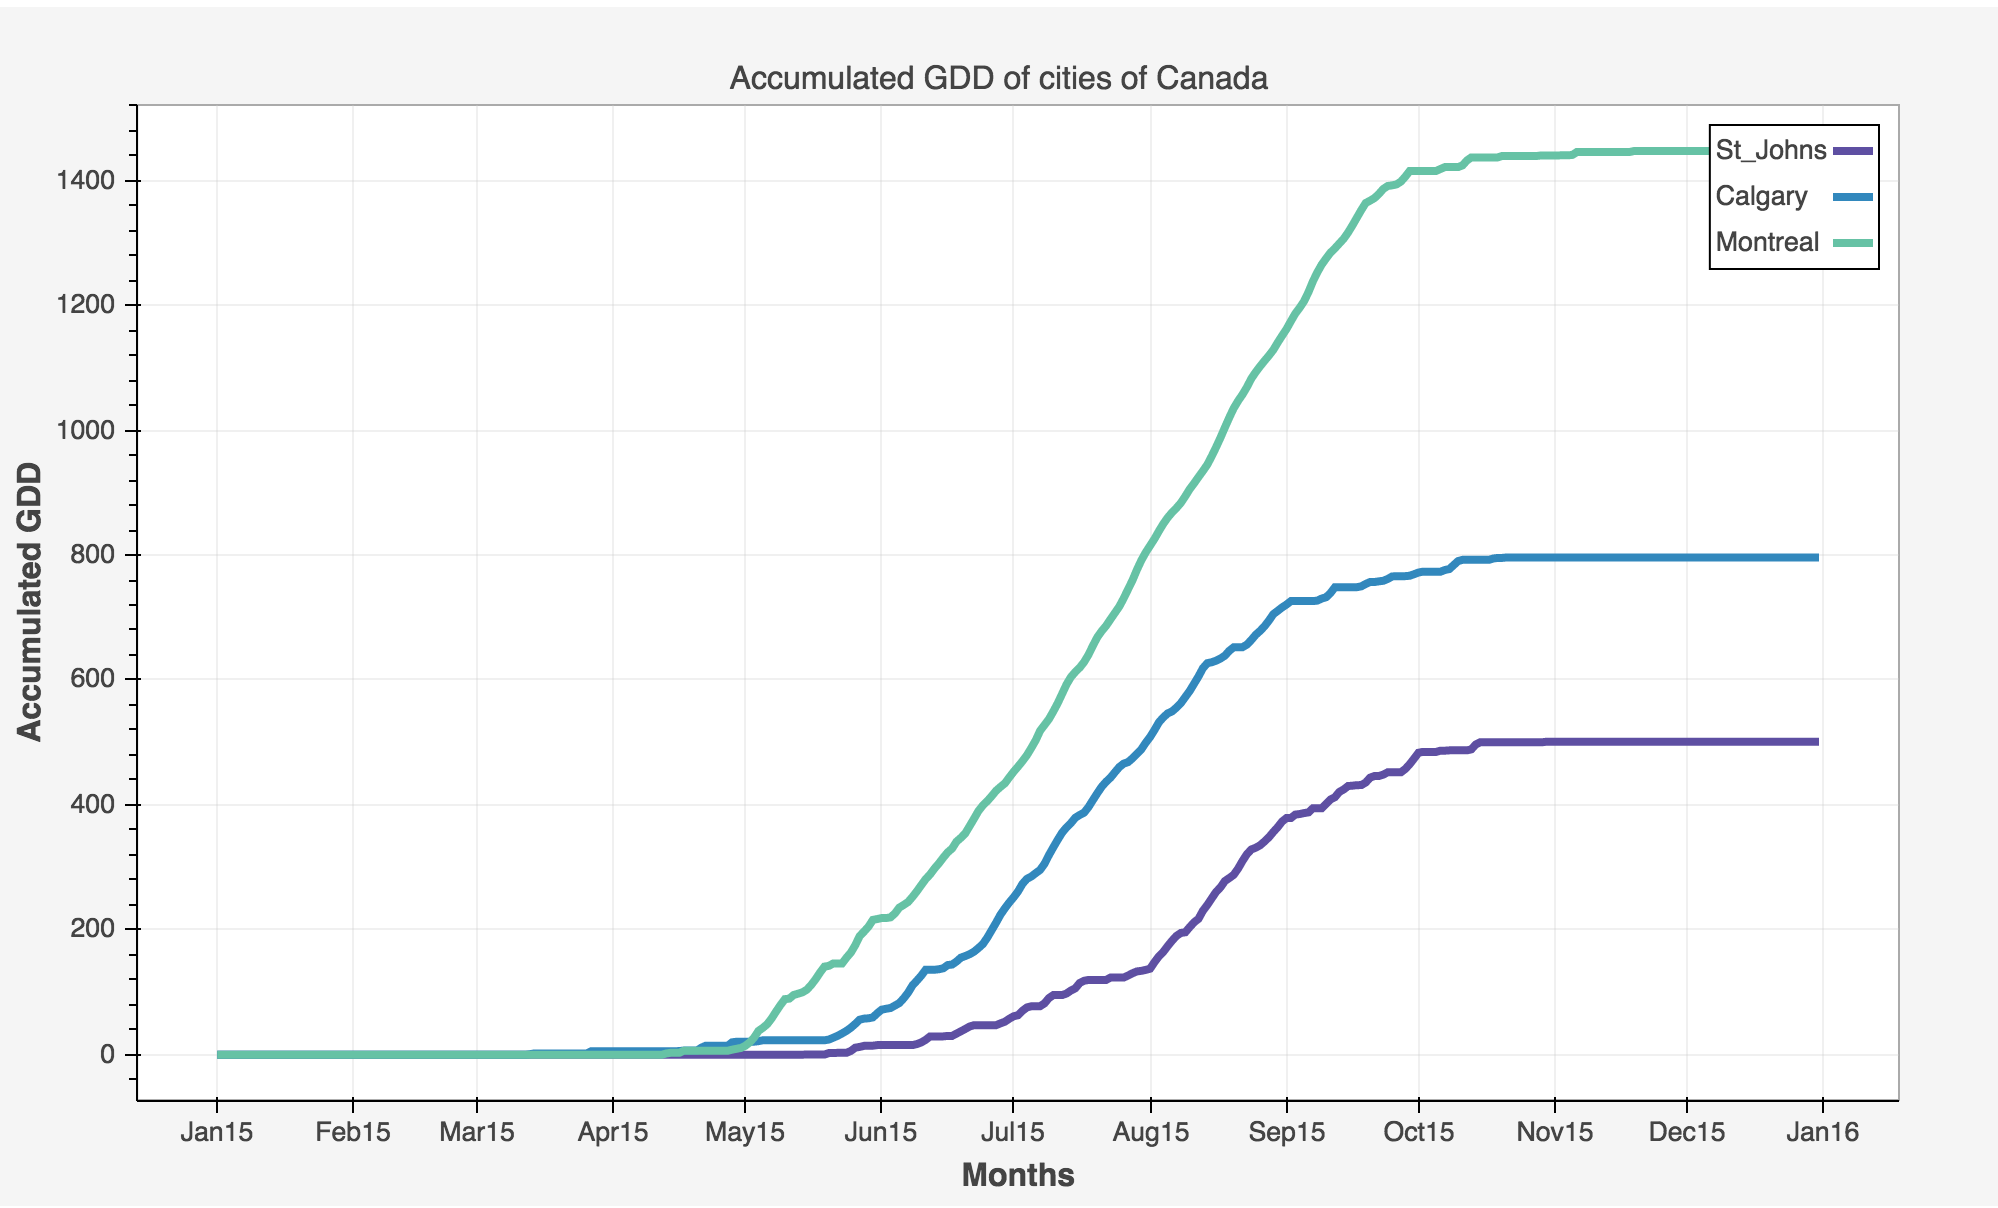
\includegraphics[width=3.25in]{./source/Report/op-task_4.png}
\caption{Interactive plot of 2015 cumulative GDD for selected cities}
\label{gdd_interactive}
\end{figure}
\end{center}

\item A bokeh server plot for visualization of accumulated GDD for any city in Canada (Fig. \ref{bokeh-server-plot_sj})

\begin{center}
\begin{figure}
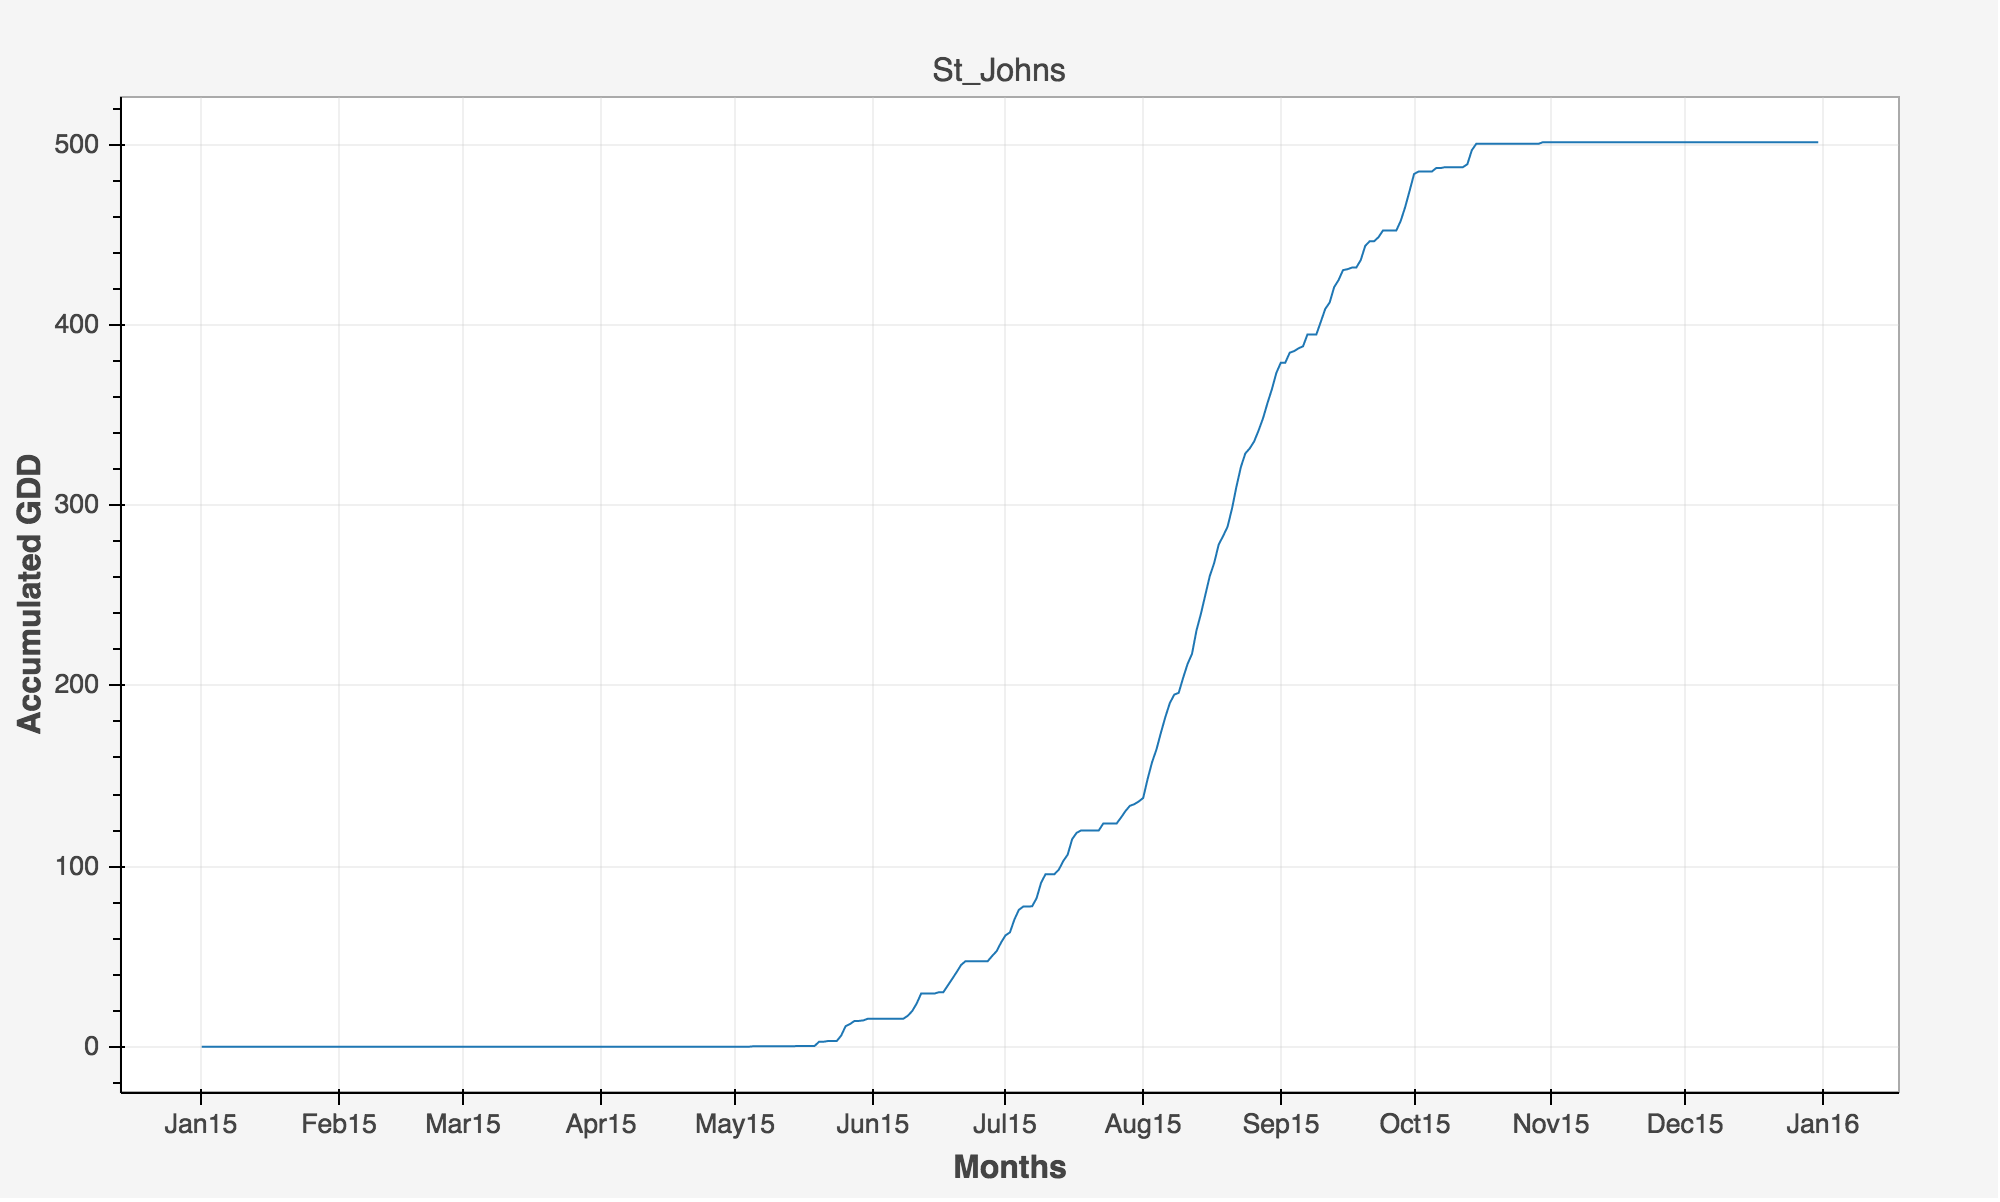
\includegraphics[width=3.25in]{./source/Report/op-task_5.png}
\caption{Bokeh server plot of 2015 cumulative GDD for St. John's}
\label{bokeh-server-plot_sj}
\end{figure}
\end{center}

\item Exploration of some aspect of the GDD dataset using analysis and visualization tools
\end{enumerate}

Comprehensive details of project tasks, files, and GDD data plots can be found in a public github repository: https://github.com/sheykholeslam/P6950T3. 


\section{ \bf Results}
A summary of the results obtained for the cumulative GDD of the selected cities is presented in Tab. \ref{gdd-results}. Fig. \ref{gdd_ann-cycle} shows the annual cumulative GDD for the three selected cities. The results indicate that the city of Montreal recorded the highest GDD value of 1448 $^{\circ}$C among the cities selected for the year 2015. The lowest cummulative GDD value of 501 $^{\circ}$C was recorded for the city of St. John's while the city of Calgary recorded a moderate cummulative GDD value of 796 $^{\circ}$C. The results suggest that among the selected cities, the city of Montreal had the warmest temperature while St. John's had the coolest temperature. Figure (\ref{gdd_min-max}) displays a plot showing the 2015 annual cycle of minimum and maximum daily temperatures for the selected cities.

\begin{table}[h]
\caption{Cumulative GDD values for selected cities in 2015} 
\label{gdd-results}
\centering
\begin{tabular}{l c}
\hline
\textbf{Cities} & \textbf{Cum. GDD} \textbf($^{\circ}$C) \\
\hline
St. John's & 501 \\
Calgary & 796 \\
Montreal & 1448 \\
\hline
\end{tabular}
\end{table}


\section{Conclusion}
The daily GDD of three cities in Canada (St. John's, Montreal and Calgary) were calculated for the year 2015. The summation of the daily GDD units were used to compare heat accumulation in these cities. The results obtained indicate that the city of Montreal had the highest cumulative GDD of 1448 $^{\circ}$C for the year 2015 among the selected cities. The city of St. John's had the lowest GDD of 501 $^{\circ}$C, while Calgary had a moderate GDD of 796 $^{\circ}$C.

\section{References}
%\bibliographystyle{plain}
\begin{enumerate}
\item Gordon, R.; Bootsma, A. Analyses of growing degree-days for agriculture in Atlantic Canada \textbf{1993} \textit{Clim. Res.} 3: 169--179.
\item \href{url}{$https://en.wikipedia.org/wiki/Growing_degree-day$}
\end{enumerate}

%\bibliography{./source/Report/references.bib}



%\section{ \bf Software Architecture}
%\subsection{Tools Used}
%\subsubsection{Programming Language}
%\subsubsection{Version Control}
%\subsection{Components}
%\subsubsection{Makefile}
%\subsubsection{Plots}
%\subsubsection{Report}
%\subsubsection{Presentation}

%\section{ \bf Core Tasks}
%\subsection{Download daily historical temperature data for several cities}
%\subsection{Create a plot showing an annual cycle of min/max daily temperatures. Do this for at least three selected Canadian cities.}
%\subsection{A command line program that takes arguments.}
%This program should calculate the GDD. Internally your program should handle the command line arguments and implement the actual calculation as one or more functions. The output from this program needs to be persistently stored. Your choice on how to implement this storage. Later steps in your work flow must use the results of these calculations.
%\subsection{Create plots showing accumulated GDD vs time for selected cities}

%\subsection{Use version control (git) and collaboration tools (GitHub)}
%\subsection{Create a LaTeX report summarizing the results of your project}
%\subsection{Create a web based presentation for your results}
%\subsection{Implement your entire workflow as a Makefile. Ensure that your entire project is reproducible}
%\subsection{Create a test-suite (using the Python package nose) to demonstrate your GDD calculation works as intended}
%\subsection{Project should include adequate documentation both with your source code and Readme.md file}


%\section{ \bf Optional Tasks}
%\subsection{Create an plot showing GDD like the example below for selected Canadian cities}
%\subsection{Create a map showing effective growing degrees over both all of Canada and only for the island of Newfoundland.}
%\subsection{Explore how GDD calculation depends on the choice of $T_{base}$. show your results for either selected cities or create maps}
%\subsection{Create standalone bokeh plots embeded in your HTML presentation}
%\subsection{Create a bokeh server plot so that you can look at the accumulated GDD for any city in Canada.}



%\section{Conclusion}
%The daily GDD of three cities in Canada (St. John's, Montreal and Calgary) were calculated for the year 2015. The summation of the daily GDD units were used to compare heat accumulation in these cities. The results obtained indicate that the city of Montreal had the highest cumulative GDD of 1448 $^{\circ}$C for the year 2015 among the selected cities. The city of St. John's had the lowest GDD of 501 $^{\circ}$C, while Calgary had a moderate GDD of 796 $^{\circ}$C.

%\bibliographystyle{plain}
%\bibliography{./source/Report/references.bib}

%\begin{figure}[h!]
%\centering
%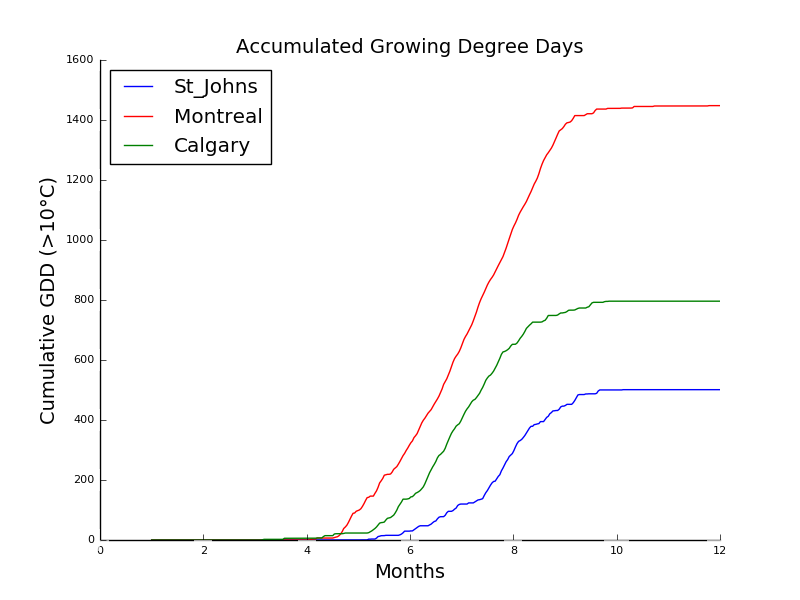
\includegraphics[scale=.5]{./Plots/GDD_Plot.png}
%\caption{GDD Cumulative Plot}
%\label{fig: GDD Plot}
%\end{figure}

\end{document}
